\section{校正方向}
\label{sec:minimax-correction}

上一节的失败发生在凸凹问题上，而且鞍点存在。所以问题不在问题本身，在迭代格式。本节先把鞍点条件写成统一的形式，看清旋转是从哪里来的，再修改迭代，用另一处的方向校正当前一步。

\paragraph{变分不等式形式}
把两组变量合并，记$\bm{z}=(\bm{x},\bm{y})$，$\bm{Z}=\bm{X}\times\bm{Y}$，定义
\begin{equation}
 \bm{F}(\bm{z})=\begin{pmatrix}\nabla_{\bm{x}}f(\bm{x},\bm{y})\\-\nabla_{\bm{y}}f(\bm{x},\bm{y})\end{pmatrix}.
 \label{eq:minimax-operator}
\end{equation}

两侧步长相同时，同时更新就是
\[
 \bm{z}^{+}=P_{\bm{Z}}\bigl(\bm{z}-\alpha\bm{F}(\bm{z})\bigr).
\]

它和投影梯度法外形一样，但$\bm{F}$一般不是任何函数的梯度。鞍点条件也能用$\bm{F}$写出来，这个写法就是第~\ref{chap:constrained-optimality}章见过的变分不等式。

\begin{theorem}[鞍点的变分不等式刻画]
\label{thm:minimax-vi}
设$\bm{X},\bm{Y}$非空闭凸，$f$在含$\bm{Z}$的开集上可微，关于$\bm{x}$凸，关于$\bm{y}$凹。则$\bm{z}^\star\in\bm{Z}$是全局鞍点，当且仅当
\begin{equation}
 \langle\bm{F}(\bm{z}^\star),\bm{z}-\bm{z}^\star\rangle\geq0\qquad\text{对所有}\ \bm{z}\in\bm{Z}.
 \label{eq:minimax-vi}
\end{equation}
\end{theorem}

\begin{proof}
记$\bm{z}^\star=(\bm{x}^\star,\bm{y}^\star)$。设它是鞍点。$\bm{x}^\star$在凸集$\bm{X}$上最小化可微凸函数$f(\cdot,\bm{y}^\star)$，一阶条件给出
\[
 \langle\nabla_{\bm{x}}f(\bm{z}^\star),\bm{x}-\bm{x}^\star\rangle\geq0.
\]
$\bm{y}^\star$在$\bm{Y}$上最大化凹函数$f(\bm{x}^\star,\cdot)$，一阶条件给出
\[
 \langle-\nabla_{\bm{y}}f(\bm{z}^\star),\bm{y}-\bm{y}^\star\rangle\geq0.
\]
两式相加即为式~\eqref{eq:minimax-vi}。

反过来，在式~\eqref{eq:minimax-vi}中取$\bm{z}=(\bm{x},\bm{y}^\star)$，得到上面第一式，由凸性，$\bm{x}^\star$是$f(\cdot,\bm{y}^\star)$的全局最小点。取$\bm{z}=(\bm{x}^\star,\bm{y})$，得到第二式，由凹性，$\bm{y}^\star$是$f(\bm{x}^\star,\cdot)$的全局最大点。这就是式~\eqref{eq:minimax-saddle}。
\end{proof}

式~\eqref{eq:minimax-vi}的几何含义是，从$\bm{z}^\star$看向任何可行方向，它与$\bm{F}(\bm{z}^\star)$的夹角都不超过直角，见图~\ref{fig:minimax-vi-geometry}。

\begin{BookInlineFigure}
 \centering
 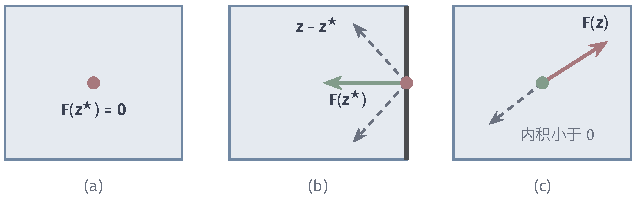
\includegraphics[width=107.7mm]{figures/05-optimization/07-multiple-criteria-and-nested-optimization/tikz/minimax-vi-geometry/figure.pdf}
 \caption{变分不等式的几何。浅蓝矩形是$\bm{Z}$。(a)解在内部时$\bm{F}(\bm{z}^\star)=\bm{0}$。(b)解在边界（深灰粗线）上时$\bm{F}(\bm{z}^\star)$指向内部，虚线表示的可行方向$\bm{z}-\bm{z}^\star$都与它成锐角。(c)绿点不是解，存在可行方向与红色的$\bm{F}(\bm{z})$内积为负。}
 \label{fig:minimax-vi-geometry}
\end{BookInlineFigure}

$\bm{F}$的性质由凸凹性决定。

\begin{lemma}[单调性]
\label{lem:minimax-monotone}
在定理~\ref{thm:minimax-vi}的条件下，$\bm{F}$是\term{单调算子}（monotone operator），即对任意$\bm{z}_1,\bm{z}_2\in\bm{Z}$，
\begin{equation}
 \langle\bm{F}(\bm{z}_1)-\bm{F}(\bm{z}_2),\bm{z}_1-\bm{z}_2\rangle\geq0.
 \label{eq:minimax-monotone}
\end{equation}
\end{lemma}

\begin{proof}
记$\bm{z}_i=(\bm{x}_i,\bm{y}_i)$。由$f(\cdot,\bm{y}_1)$和$f(\cdot,\bm{y}_2)$的凸性，
\[
 \begin{aligned}
 f(\bm{x}_2,\bm{y}_1)&\geq f(\bm{x}_1,\bm{y}_1)+\langle\nabla_{\bm{x}}f(\bm{z}_1),\bm{x}_2-\bm{x}_1\rangle,\\
 f(\bm{x}_1,\bm{y}_2)&\geq f(\bm{x}_2,\bm{y}_2)+\langle\nabla_{\bm{x}}f(\bm{z}_2),\bm{x}_1-\bm{x}_2\rangle.
 \end{aligned}
\]
由$f(\bm{x}_1,\cdot)$和$f(\bm{x}_2,\cdot)$的凹性，
\[
 \begin{aligned}
 f(\bm{x}_1,\bm{y}_2)&\leq f(\bm{x}_1,\bm{y}_1)+\langle\nabla_{\bm{y}}f(\bm{z}_1),\bm{y}_2-\bm{y}_1\rangle,\\
 f(\bm{x}_2,\bm{y}_1)&\leq f(\bm{x}_2,\bm{y}_2)+\langle\nabla_{\bm{y}}f(\bm{z}_2),\bm{y}_1-\bm{y}_2\rangle.
 \end{aligned}
\]
把四个不等式相加，函数值全部相消，整理即得式~\eqref{eq:minimax-monotone}。
\end{proof}

单调是梯度单调的推广，$f$是凸函数时$\nabla f$单调。差别在于$\bm{F}$的Jacobian不对称。$f$二阶可微时，
\[
 \bm{J}=\begin{pmatrix}\nabla^2_{\bm{x}\bm{x}}f&\nabla^2_{\bm{x}\bm{y}}f\\-\nabla^2_{\bm{y}\bm{x}}f&-\nabla^2_{\bm{y}\bm{y}}f\end{pmatrix}.
\]

对角块由凸凹性是半正定的，贡献朝向解的收缩。非对角块反对称，贡献的是旋转，它对$\langle\bm{F}(\bm{z})-\bm{F}(\bm{z}'),\bm{z}-\bm{z}'\rangle$的贡献恰好是零。$f=xy$时对角块全是零，$\bm{J}$只剩反对称部分，所以$\langle\bm{F}(\bm{z}),\bm{z}\rangle=0$。单调性在这里只说明方向不朝外，并不提供任何朝向解的分量，这就是旋转现象的代数来源。

\paragraph{校正的想法}
旋转场里，当前点的方向用一整步就过时了，走到新位置时场已经转了角度。一个自然的修补是：先试探着走一步，读取试探点处的方向，再回到原来的位置，用这个方向走一步。下面的表把这个想法和几种看起来相近的技巧放在一起。

\begin{BookInlineTable}
 \centering
 \begin{tabular}{@{}lll@{}}
  \toprule
  技巧 & 改的是什么 & 对$f=xy$的效果\\
  \midrule
  重球动量 & 叠加上一步的位移 & 把切向位移加强，更快发散\\
  乘子法 & 改目标，加增广项后解内层 & 需要解子问题\\
  外梯度 & 方向取自预测点 & 收缩\\
  乐观梯度 & 用方向的差分校正 & 收缩\\
  \bottomrule
 \end{tabular}
 \caption{几种修改迭代或目标的办法。前两种不是校正方向。}
 \label{tab:minimax-correction-compare}
\end{BookInlineTable}

重球法是第~\ref{chap:first-order-methods}章的单目标加速，叠加的是位置差$\bm{z}^{(t)}-\bm{z}^{(t-1)}$。在$f=xy$上，上一步的位移本身就是切向的，叠加之后向外偏得更多。取$\alpha=0.2$，动量系数$0.5$，迭代的谱半径是$1.125$，比不加动量时的$1.020$还大。

第~\ref{chap:penalty-multiplier-methods}章的乘子法也交替更新原变量和乘子，但它在$\bm{x}$上解一个增广Lagrange子问题，增广项改变了目标。校正方向不改$f$，只改读取方向的位置，每轮仍只是读取几次方向。

\subsection{外梯度法}
\label{sec:minimax-extragradient}

\paragraph{主要思想}
\term{外梯度法}（extragradient method，EG）每轮读取两次方向\scite{korpelevich1976}。先从当前点走一个试探步，读取新方向，再回到当前点，用新方向完成校正：
\begin{equation}
 \begin{aligned}
 \tilde{\bm{z}}^{(t)}&=P_{\bm{Z}}\bigl(\bm{z}^{(t)}-\alpha\bm{F}(\bm{z}^{(t)})\bigr),\\
 \bm{z}^{(t+1)}&=P_{\bm{Z}}\bigl(\bm{z}^{(t)}-\alpha\bm{F}(\tilde{\bm{z}}^{(t)})\bigr).
 \end{aligned}
 \label{eq:minimax-eg}
\end{equation}

校正步的起点仍是$\bm{z}^{(t)}$，只是方向换成了试探点的方向。这和连续做两次普通梯度步不同，后者的第二步从$\tilde{\bm{z}}^{(t)}$出发。

为什么这样能收缩？看$f=xy$，$\bm{F}(x,y)=(y,-x)$。在图~\ref{fig:minimax-eg-step}中，从$\bm{z}$沿切线走到$\tilde{\bm{z}}$，那里的方向已经向内转过了一个角度。把这个方向拿回$\bm{z}$，迈出的一步就略微朝向圆内，抵消了切线外漂。

\begin{BookInlineFigure}
 \centering
 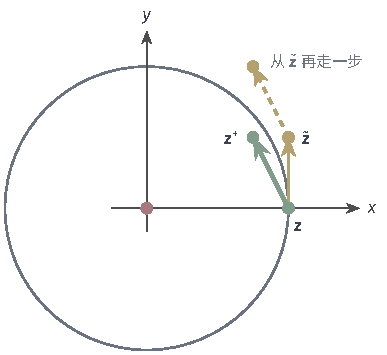
\includegraphics[width=65.6mm]{figures/05-optimization/07-multiple-criteria-and-nested-optimization/tikz/minimax-eg-step/figure.pdf}
 \caption{外梯度的一步，$f=xy$，$\alpha=\frac12$。灰色圆是过$\bm{z}=(1,0)$的等距圆，红点是鞍点。黄色实线箭头走到试探点$\tilde{\bm{z}}=(1,0.5)$，绿色箭头从$\bm{z}$沿试探点的方向走到$\bm{z}^{+}=(0.75,0.5)$，落在圆内。黄色虚线是从试探点再走一步普通梯度步，到$(0.75,1)$，落在圆外。}
 \label{fig:minimax-eg-step}
\end{BookInlineFigure}

代数上，把$\bm{F}(\bm{z})=\bm{A}\bm{z}$代入，$\bm{A}=\begin{pmatrix}0&1\\-1&0\end{pmatrix}$，得到
\[
 \bm{z}^{+}=\bm{z}-\alpha\bm{A}(\bm{z}-\alpha\bm{A}\bm{z})=\bigl(\bm{I}-\alpha\bm{A}+\alpha^2\bm{A}^2\bigr)\bm{z}.
\]

由于$\bm{A}^2=-\bm{I}$，上式成为$\bm{z}^{+}=(1-\alpha^2)\bm{z}-\alpha\bm{A}\bm{z}$。$\bm{z}$与$\bm{A}\bm{z}$正交，长度相同，所以
\begin{equation}
 \lVert\bm{z}^{+}\rVert_2^2=\bigl(1-\alpha^2+\alpha^4\bigr)\lVert\bm{z}\rVert_2^2.
 \label{eq:minimax-eg-contraction}
\end{equation}
$0<\alpha<1$时这个因子小于$1$。多读取的那一次方向，把式~\eqref{eq:minimax-gda-growth}里的$+\alpha^2$换成了$-\alpha^2$，这是二阶项的差别。

\paragraph{计算过程}
用$f=xy$，$X=Y=\mathbb{R}$，投影是恒等映射。

\needspace{6\baselineskip}
\paragraph{变量}
\begin{itemize}
 \item $\bm{z}^{(t)}=(x^{(t)},y^{(t)})$：当前点；
 \item $\tilde{\bm{z}}^{(t)}$：试探点；
 \item $\alpha>0$：步长。
\end{itemize}

\paragraph{初始化}
取$\bm{z}^{(0)}\in\bm{Z}$。例中$\bm{z}^{(0)}=(1,0)$，$\alpha=\frac12$，与上一节相同，便于比较。

\needspace{6\baselineskip}
\paragraph{每轮更新}
\begin{enumerate}
 \item 在当前点读取方向并试探。例中第一轮
 \[
  \bm{F}(\bm{z}^{(0)})=(0,-1),\qquad\tilde{\bm{z}}^{(0)}=(1,0)-\frac12(0,-1)=(1,0.5).
 \]
 \item 在试探点读取方向，回到当前点校正。例中第一轮
 \[
  \bm{F}(\tilde{\bm{z}}^{(0)})=(0.5,-1),\qquad\bm{z}^{(1)}=(1,0)-\frac12(0.5,-1)=(0.75,0.5).
 \]
\end{enumerate}

第二轮的试探和校正分别是
\[
 \tilde{\bm{z}}^{(1)}=(0.5,0.875),\qquad\bm{z}^{(2)}=(0.3125,0.75).
\]
距离的平方依次为$1,0.8125,0.6602$，每轮乘以$0.8125=1-\frac14+\frac1{16}$，与式~\eqref{eq:minimax-eg-contraction}一致。通常在残差或步数达到要求时结束。最终得到的迭代点向鞍点几何收敛，而同样步长的同时更新每轮乘以$1.25$。

\paragraph{平均点的间隙保证}
双线性例子的收缩依赖具体的矩阵。一般问题上，外梯度法的保证来自单调性和Lipschitz性，对象是试探点的平均
\[
 \hat{\bm{z}}_T=(\hat{\bm{x}}_T,\hat{\bm{y}}_T)=\frac1T\sum_{t=0}^{T-1}\tilde{\bm{z}}^{(t)}.
\]

证明用到投影的刻画：$\bm{p}=P_{\bm{Z}}(\bm{w})$当且仅当$\bm{p}\in\bm{Z}$，且
\begin{equation}
 \langle\bm{w}-\bm{p},\bm{u}-\bm{p}\rangle\leq0\qquad\text{对所有}\ \bm{u}\in\bm{Z}.
 \label{eq:minimax-projection}
\end{equation}

\begin{theorem}[外梯度法的平均间隙]
\label{thm:minimax-eg-gap}
设$\bm{Z}=\bm{X}\times\bm{Y}$非空、紧、凸，直径为$D$；$f$在含$\bm{Z}$的开集上可微，关于$\bm{x}$凸，关于$\bm{y}$凹；$\bm{F}$在$\bm{Z}$上$L$-Lipschitz，$0<\alpha\leq1/L$。则对任意$T\geq1$，
\begin{equation}
 G(\hat{\bm{x}}_T,\hat{\bm{y}}_T)\leq\frac{D^2}{2\alpha T}.
 \label{eq:minimax-eg-gap}
\end{equation}
\end{theorem}

\begin{proof}
固定$\bm{v}=(\bm{x},\bm{y})\in\bm{Z}$，一轮内省略上标，记$\bm{z},\tilde{\bm{z}},\bm{z}^{+}$，$\tilde{\bm{F}}=\bm{F}(\tilde{\bm{z}})$。

对校正步用式~\eqref{eq:minimax-projection}，取$\bm{w}=\bm{z}-\alpha\tilde{\bm{F}}$，$\bm{p}=\bm{z}^{+}$，$\bm{u}=\bm{v}$，整理得
\[
 \alpha\langle\tilde{\bm{F}},\bm{z}^{+}-\bm{v}\rangle\leq\langle\bm{z}-\bm{z}^{+},\bm{z}^{+}-\bm{v}\rangle.
\]
对试探步用式~\eqref{eq:minimax-projection}，取$\bm{w}=\bm{z}-\alpha\bm{F}(\bm{z})$，$\bm{p}=\tilde{\bm{z}}$，$\bm{u}=\bm{z}^{+}$，整理得
\[
 \alpha\langle\bm{F}(\bm{z}),\tilde{\bm{z}}-\bm{z}^{+}\rangle\leq\langle\bm{z}-\tilde{\bm{z}},\tilde{\bm{z}}-\bm{z}^{+}\rangle.
\]

把要估计的内积拆成三项：
\[
 \begin{aligned}
 \alpha\langle\tilde{\bm{F}},\tilde{\bm{z}}-\bm{v}\rangle
 ={}&\alpha\langle\tilde{\bm{F}},\bm{z}^{+}-\bm{v}\rangle+\alpha\langle\bm{F}(\bm{z}),\tilde{\bm{z}}-\bm{z}^{+}\rangle\\
 &+\alpha\langle\tilde{\bm{F}}-\bm{F}(\bm{z}),\tilde{\bm{z}}-\bm{z}^{+}\rangle.
 \end{aligned}
\]

对任意向量有恒等式
\[
 2\langle\bm{a}-\bm{b},\bm{b}-\bm{c}\rangle=\lVert\bm{a}-\bm{c}\rVert_2^2-\lVert\bm{a}-\bm{b}\rVert_2^2-\lVert\bm{b}-\bm{c}\rVert_2^2.
\]
用它处理前两项的上界：
\[
 \begin{aligned}
 2\langle\bm{z}-\bm{z}^{+},\bm{z}^{+}-\bm{v}\rangle&=\lVert\bm{z}-\bm{v}\rVert_2^2-\lVert\bm{z}-\bm{z}^{+}\rVert_2^2-\lVert\bm{z}^{+}-\bm{v}\rVert_2^2,\\
 2\langle\bm{z}-\tilde{\bm{z}},\tilde{\bm{z}}-\bm{z}^{+}\rangle&=\lVert\bm{z}-\bm{z}^{+}\rVert_2^2-\lVert\bm{z}-\tilde{\bm{z}}\rVert_2^2-\lVert\tilde{\bm{z}}-\bm{z}^{+}\rVert_2^2.
 \end{aligned}
\]

第三项由Cauchy--Schwarz、Lipschitz条件、$\alpha L\leq1$和$2ab\leq a^2+b^2$控制：
\[
 2\alpha\langle\tilde{\bm{F}}-\bm{F}(\bm{z}),\tilde{\bm{z}}-\bm{z}^{+}\rangle\leq\lVert\tilde{\bm{z}}-\bm{z}\rVert_2^2+\lVert\tilde{\bm{z}}-\bm{z}^{+}\rVert_2^2.
\]

三项相加，$\lVert\bm{z}-\bm{z}^{+}\rVert_2^2$、$\lVert\bm{z}-\tilde{\bm{z}}\rVert_2^2$和$\lVert\tilde{\bm{z}}-\bm{z}^{+}\rVert_2^2$全部相消，得到
\[
 2\alpha\langle\tilde{\bm{F}},\tilde{\bm{z}}-\bm{v}\rangle\leq\lVert\bm{z}-\bm{v}\rVert_2^2-\lVert\bm{z}^{+}-\bm{v}\rVert_2^2.
\]

对$t=0,\ldots,T-1$求和，右端逐项相消，不超过$\lVert\bm{z}^{(0)}-\bm{v}\rVert_2^2\leq D^2$。

再把内积换成函数值。记$\tilde{\bm{z}}=(\tilde{\bm{x}},\tilde{\bm{y}})$。由$f(\cdot,\tilde{\bm{y}})$的凸性和$f(\tilde{\bm{x}},\cdot)$的凹性，
\[
 \begin{aligned}
 \langle\nabla_{\bm{x}}f(\tilde{\bm{z}}),\tilde{\bm{x}}-\bm{x}\rangle&\geq f(\tilde{\bm{x}},\tilde{\bm{y}})-f(\bm{x},\tilde{\bm{y}}),\\
 \langle-\nabla_{\bm{y}}f(\tilde{\bm{z}}),\tilde{\bm{y}}-\bm{y}\rangle&\geq f(\tilde{\bm{x}},\bm{y})-f(\tilde{\bm{x}},\tilde{\bm{y}}).
 \end{aligned}
\]
两式相加，得到
\[
 \langle\tilde{\bm{F}},\tilde{\bm{z}}-\bm{v}\rangle\geq f(\tilde{\bm{x}},\bm{y})-f(\bm{x},\tilde{\bm{y}}).
\]

对$t$取平均。由Jensen不等式，$f(\cdot,\bm{y})$凸，所以平均点的值不超过值的平均；$f(\bm{x},\cdot)$凹，所以平均点的值不低于值的平均。于是
\[
 f(\hat{\bm{x}}_T,\bm{y})-f(\bm{x},\hat{\bm{y}}_T)\leq\frac{D^2}{2\alpha T}.
\]
此式对所有$\bm{y}\in\bm{Y}$和$\bm{x}\in\bm{X}$成立。左端对$\bm{y}$取最大、对$\bm{x}$取最小，就是$G(\hat{\bm{x}}_T,\hat{\bm{y}}_T)$。
\end{proof}

这里的$\bm{Z}$需要紧，否则$D$无穷，间隙也可能无穷。证明里真正起作用的是单调性和Lipschitz性，不是“多算一次梯度”这个动作本身。所以这个保证不能搬到非凸非凹的问题上。

计算代价方面，每轮要读取两次$\bm{F}$、做两次投影，是同时更新的两倍。比较时应按读取次数，而不是轮数。图~\ref{fig:minimax-eg-paths}按读取次数画出了三种方法，其中紫线是下一小节的方法。

\begin{BookInlineFigure}
 \centering
 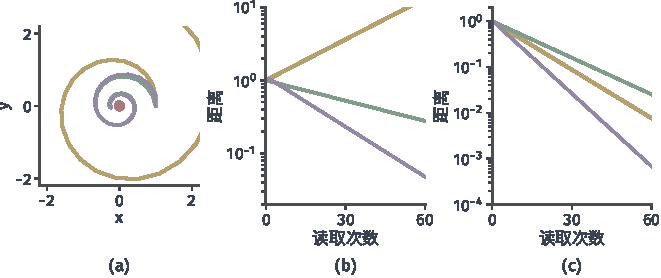
\includegraphics[width=112mm]{figures/05-optimization/07-multiple-criteria-and-nested-optimization/matplotlib/minimax-eg-paths/figure.pdf}
 \caption{三种方法的比较：黄线同时更新，绿线外梯度，紫线乐观梯度，起点$(1,0)$。(a)$f=xy$，$\alpha=0.3$，$30$轮的轨迹，红点是解。(b)$f=xy$到解的距离，横轴是方向读取次数，外梯度每轮计$2$次。(c)$f=\frac12x^2+2xy-\frac12y^2$，$\alpha=0.1$，同样按读取次数。}
 \label{fig:minimax-eg-paths}
\end{BookInlineFigure}

\subsection{乐观梯度法}
\label{sec:minimax-ogda}

\paragraph{主要思想}
外梯度法每轮读两次方向，能不能省一次？试探步的目的只是估计“下一步的方向”，而上一轮刚读过的方向已经是一个不错的估计。把试探步里的方向换成上一轮的$\bm{F}(\tilde{\bm{z}}^{(t-1)})$，无约束时得到
\[
 \tilde{\bm{z}}^{(t)}=\bm{z}^{(t)}-\alpha\bm{F}(\tilde{\bm{z}}^{(t-1)}),\qquad\bm{z}^{(t+1)}=\bm{z}^{(t)}-\alpha\bm{F}(\tilde{\bm{z}}^{(t)}).
\]
每轮只新读$\bm{F}(\tilde{\bm{z}}^{(t)})$一次。

把这个递推写成只含$\tilde{\bm{z}}$的形式。下一轮的试探点是
\[
 \tilde{\bm{z}}^{(t+1)}=\bm{z}^{(t+1)}-\alpha\bm{F}(\tilde{\bm{z}}^{(t)})=\bm{z}^{(t)}-2\alpha\bm{F}(\tilde{\bm{z}}^{(t)}).
\]
又由试探步，
\[
 \bm{z}^{(t)}=\tilde{\bm{z}}^{(t)}+\alpha\bm{F}(\tilde{\bm{z}}^{(t-1)}).
\]
代入后把$\tilde{\bm{z}}$重新记作$\bm{z}$，得到\term{乐观梯度下降—上升}（optimistic gradient descent--ascent，OGDA）：
\begin{equation}
 \bm{z}^{(t+1)}=\bm{z}^{(t)}-2\alpha\bm{F}(\bm{z}^{(t)})+\alpha\bm{F}(\bm{z}^{(t-1)}).
 \label{eq:minimax-ogda}
\end{equation}

把它写成
\[
 \bm{z}^{(t+1)}=\bm{z}^{(t)}-\alpha\bm{F}(\bm{z}^{(t)})-\alpha\bigl(\bm{F}(\bm{z}^{(t)})-\bm{F}(\bm{z}^{(t-1)})\bigr)
\]
就能看出它的含义。括号里是方向场在上一步中的变化量，代表耦合带来的转动。它按当前的变化趋势，把下一步的方向提前校正。“乐观”指相信方向场短期内的变化趋势会延续。它与重球动量的区别在于，重球叠加的是位置的差，这里叠加的是方向的差。

\paragraph{计算过程}
用$f=xy$，$\bm{F}(x,y)=(y,-x)$。

\needspace{6\baselineskip}
\paragraph{变量}
\begin{itemize}
 \item $\bm{z}^{(t)}$：当前点；
 \item $\bm{F}^{(t-1)}$：上一轮读到的方向，需要存储；
 \item $\alpha>0$：步长。
\end{itemize}

\paragraph{初始化}
取$\bm{z}^{(0)}$，并令$\bm{z}^{(-1)}=\bm{z}^{(0)}$，于是第一步就是普通的梯度步。例中$\bm{z}^{(0)}=(1,0)$，$\alpha=0.2$。

\needspace{6\baselineskip}
\paragraph{每轮更新}
\begin{enumerate}
 \item 读取当前方向$\bm{F}^{(t)}=\bm{F}(\bm{z}^{(t)})$。例中第一轮$\bm{F}^{(0)}=(0,-1)$，第二轮
 \[
  \bm{z}^{(1)}=(1,0.2),\qquad\bm{F}^{(1)}=(0.2,-1).
 \]
 \item 由式~\eqref{eq:minimax-ogda}更新，并保存$\bm{F}^{(t)}$。例中第二轮
 \[
  \bm{z}^{(2)}=(1,0.2)-0.4(0.2,-1)+0.2(0,-1)=(0.92,0.4).
 \]
\end{enumerate}

继续计算，得到
\[
 \bm{z}^{(3)}=(0.8,0.568),\qquad\bm{z}^{(4)}=(0.6528,0.704).
\]
距离的平方依次为$1,1.04,1.0064,0.9626,0.9218$，第一步因为没有历史而外漂，之后开始收缩。最终得到的迭代点沿螺旋线趋向鞍点，每轮只读一次方向。

\paragraph{双线性情形的稳定性}
线性的$\bm{F}$可以算到底。把$(x,y)$看作复数$w=x+\mathrm{i}y$，$\bm{F}=(y,-x)$对应$-\mathrm{i}w$，同时更新就成了$w^{+}=(1+\mathrm{i}\alpha)w$，与式~\eqref{eq:minimax-gda-growth}一致。式~\eqref{eq:minimax-ogda}成为二阶递推
\[
 w^{(t+1)}=(1+2\mathrm{i}\alpha)w^{(t)}-\mathrm{i}\alpha w^{(t-1)}.
\]
它的特征方程是$s^2-(1+2\mathrm{i}\alpha)s+\mathrm{i}\alpha=0$，判别式是
\[
 (1+2\mathrm{i}\alpha)^2-4\mathrm{i}\alpha=1-4\alpha^2.
\]

$0<\alpha\leq\frac12$时判别式非负，两根是$\frac12(1+2\mathrm{i}\alpha\pm\sqrt{1-4\alpha^2})$，模较大的那个满足
\begin{equation}
 \rho^2=\frac{1+\sqrt{1-4\alpha^2}}{2}<1.
 \label{eq:minimax-ogda-bilinear}
\end{equation}

$\alpha=0.2$时$\rho^2\approx0.958$，上面逐步算出的距离确实以这个比例下降。小步长时$\rho^2\approx1-\alpha^2$，和外梯度的式~\eqref{eq:minimax-eg-contraction}同阶。$\alpha>\frac12$时两根的虚部不同，由$\lvert s\rvert^2<1$可得稳定的条件是$\alpha<1/\sqrt{3}\approx0.577$，见图~\ref{fig:minimax-ogda-stability}(a)。外梯度的范围更宽，到$\alpha<1$。

\begin{BookInlineFigure}
 \centering
 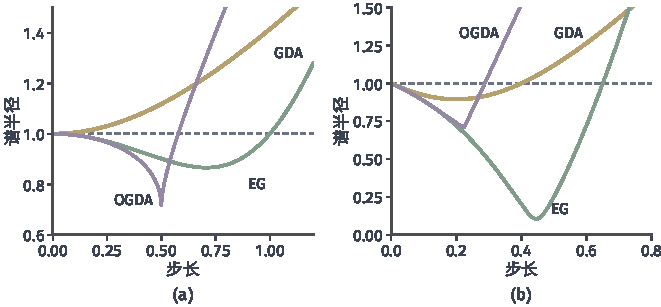
\includegraphics[width=112mm]{figures/05-optimization/07-multiple-criteria-and-nested-optimization/matplotlib/minimax-ogda-stability/figure.pdf}
 \caption{线性$\bm{F}$上的谱半径与步长的关系。虚线是稳定边界$1$。(a)$f=xy$：同时更新（GDA）全在边界之上。外梯度（EG）到$\alpha<1$稳定，乐观梯度（OGDA）到$\alpha<0.577$稳定。(b)$f=\frac12x^2+2xy-\frac12y^2$：三种方法都有稳定区间，分别到$0.4$、$0.65$、$0.29$。}
 \label{fig:minimax-ogda-stability}
\end{BookInlineFigure}

\paragraph{强凸—强凹情形}
取$f=\frac12x^2+2xy-\frac12y^2$，关于$x$强凸，关于$y$强凹，$\mu=1$。$\bm{F}$是线性的，其矩阵的特征值和Lipschitz常数是
\[
 \lambda=1\pm2\mathrm{i},\qquad L=\lvert\lambda\rvert=\sqrt5.
\]

同时更新和外梯度的每轮因子分别是$\lvert1-\alpha\lambda\rvert$和$\lvert1-\alpha\lambda+\alpha^2\lambda^2\rvert$。乐观梯度的因子是下面方程模较大的根：\[
 s^2-(1-2\alpha\lambda)s-\alpha\lambda=0.
\]

\begin{BookInlineTable}
 \centering
 \begin{tabular}{@{}llll@{}}
  \toprule
  方法 & $\alpha=0.1$ & $\alpha=0.2$ & 稳定上限\\
  \midrule
  GDA & $0.922$ & $0.894$ & $0.400$\\
  EG & $0.885$ & $0.721$ & $0.651$\\
  OGDA & $0.885$ & $0.739$ & $0.288$\\
  \bottomrule
 \end{tabular}
 \caption{$f=\frac12x^2+2xy-\frac12y^2$上三种方法的每轮收缩因子及步长上限（数值求得）。}
 \label{tab:minimax-sc-rates}
\end{BookInlineTable}

表~\ref{tab:minimax-sc-rates}的因子是按轮计算的，外梯度每轮读两次方向。按读取次数折算，$\alpha=0.1$时外梯度相当于每次读取收缩$\sqrt{0.885}\approx0.941$，比同时更新的$0.922$还慢，图~\ref{fig:minimax-eg-paths}(c)里绿线在黄线之上就是这个原因。外梯度的优势要靠较大的步长才能体现，图~\ref{fig:minimax-ogda-stability}(b)中它在$\alpha\approx0.45$处的每轮因子只有$0.105$。

对一般的强单调、Lipschitz算子，已知结论是外梯度和乐观梯度取$\alpha$为$1/L$量级时，每轮收缩因子是$1-O(\mu/L)$，而同时更新的步长要小到$\mu/L^2$量级，因子是$1-O(\mu^2/L^2)$。证明需要构造带历史项的势函数，篇幅较长，读者可查阅专门的变分不等式著作。

\paragraph{不能直接推广的情形}
上述核对都在单调问题上。$f=y^2-x^2$的$\bm{F}=(-2x,-2y)$，$\lambda=-2$，原点是排斥的：式~\eqref{eq:minimax-ogda}的特征方程$s^2-(1+4\alpha)s+2\alpha=0$在$s=1$处取值$-2\alpha<0$，所以有一根大于$1$。同样的计算也使外梯度的因子$1+2\alpha+4\alpha^2$大于$1$。

有约束时还要分清变体。把投影直接加到式~\eqref{eq:minimax-ogda}上，得到$P_{\bm{Z}}(\bm{z}^{(t)}-2\alpha\bm{F}(\bm{z}^{(t)})+\alpha\bm{F}(\bm{z}^{(t-1)}))$；另一种形式保留试探点和校正点两条序列，各做一次投影。无约束时二者等价，有约束时不是同一个递推。

例如在盒子$[-1,1]^2$上，$\bm{z}^{(0)}=(1,0.9)$，$\alpha=0.4$，$\bm{F}=(y,-x)$，第一步前者给出$(0.64,1)$，后者给出$(0.6,1)$。两种形式的步长条件和分析要分别核对，不能把其中一种的保证直接用到另一种，更不能推广到任意的非凸问题。
